\begin{frame}
	\begin{center}
		\Huge
		\textbf{Appendix}
	\end{center}
\end{frame}
\begin{frame}
	\frametitle{Robustness Study}
	\begin{figure}
		\vspace{-0.5cm}
		\centering
		\subfloat[Degree 2, shift $-0.06$]{\includegraphics[width=0.45\textwidth]{img/2_2.png}}
		\subfloat[Degree 2, shift $-0.03$]{\includegraphics[width=0.45\textwidth]{img/2_4.png}}
	\end{figure}
	\begin{itemize}
		\item Visualised agglomerated cells
	\end{itemize}
\end{frame}	
\begin{frame}
	\frametitle{Degrees of Freedom for Viscid Simulations}
	\begin{table}[htp]
		\centering
		\def\arraystretch{1.5}
		\begin{tabular}{|c|c|c|c|c|}
			\hline
			\multicolumn{2}{|c|}{\multirow{2}{*}{DoFs}} & \multicolumn{3}{c|}{CpD} \\ \cline{3-5} 
			\multicolumn{2}{|c|}{}                       & 40     & 60    & 80    \\ \hline
			\multirow{3}{*}{DG}            & 1           &    4800    &    10800   &    19200    \\ \cline{2-5} 
			& 2           &    9600    &   21600    &    38400    \\ \cline{2-5} 
			& 3           &      16000  &   36000    &   64000     \\ \hline
		\end{tabular}
		\caption{Degrees of Freedom for Different Simulation Properties}	
		\label{DOF}
	\end{table}
\end{frame}	
\begin{frame}[allowframebreaks]
	\frametitle{Values for $\text{Re}=20$}
	\begin{columns}
		\column{6cm}
		\begin{table}[htp]
			\centering
			\def\arraystretch{1.5}
			%	\begin{minipage}[b]{0.3\textwidth}	
			\begin{tabular}{|c|c|c|c|c|}
				\hline
				\multicolumn{2}{|c|}{\multirow{2}{*}{$C_D$}} & \multicolumn{3}{c|}{CpD} \\ \cline{3-5} 
				\multicolumn{2}{|c|}{}                       & 40     & 60    & 80    \\ \hline
				\multirow{3}{*}{DG}            & 1           &    $1.812$    &  $1.952$     &    $1.988$    \\ \cline{2-5} 
				& 2           &    $2.141$    &    $2.138$   &   $2.197$     \\ \cline{2-5} 
				& 3           &    $2.136$    &     $2.136$  &   -     \\ \hline
			\end{tabular}
			\caption[$C_D$ Values for Each Simulation]{$C_D$ Values for Each Simulation ($\text{Re} = 20$)}	
			\label{C_D20}
		\end{table}
		\column{6cm}
			\begin{table}[htp]
				\centering
				\def\arraystretch{1.5}
				%	\end{minipage}
				%	\centering
				%	\quad
				%	\begin{minipage}[b]{0.3\textwidth}	
				\begin{tabular}{|c|c|c|c|c|}
					\hline
					\multicolumn{2}{|c|}{\multirow{2}{*}{$W^*$}} & \multicolumn{3}{c|}{CpD} \\ \cline{3-5} 
					\multicolumn{2}{|c|}{}                       & 40     & 60    & 80    \\ \hline
					\multirow{3}{*}{DG}            & 1           &    $0.956$    &     $1.044$  &    $0.927$    \\ \cline{2-5} 
					& 2           &    $0.887$    &     $0.943$  &    $0.916$    \\ \cline{2-5} 
					& 3           &     $0.921$   &     $0.928$  &    -    \\ \hline
				\end{tabular}
				\caption{Wake Separation Lengths for Each Simulation ($\text{Re} = 20$)}	
				\label{W20}
				%	\end{minipage}
			\end{table}		
	\end{columns}
		\scalebox{0.8}{
			\begin{minipage}{\the\textwidth}
\begin{figure}[htp]	
	\centering
	\begin{tikzpicture}
	\begin{semilogyaxis}[xlabel ={Time}, ylabel ={$C_D$},  grid =major, unbounded coords=jump, legend style = {cells = {anchor=east}, legend pos=outer north east}, scaled x ticks = false, scaled y ticks = false, xmin = 0, xmax = 14]
	\addplot[brown] table[x = t, y =C_D, mark=none] {data/re20dg1cpd40.dat};
	\addlegendentry{DG1CpD40}
	\addplot[red] table[ x = t, y =C_D, mark=none] {data/re20dg2cpd60.dat};
	\addlegendentry{DG2CpD60}
	\addplot[blue] table[ x = t, y =C_D, mark=none] {data/re20dg3cpd60.dat};
	\addlegendentry{DG3CpD60}
	\addplot[black] table[ x = t, y =C_D, mark=none] {data/re20dg2cpd80.dat};
	\addlegendentry{DG2CpD80}
	%		\addplot[mark=none, red] coordinates {(32, 1.6) (128, 1.6)};
	%		\addlegendentry{Constant Value}
	\end{semilogyaxis}	
	\end{tikzpicture}
	\caption{Coefficient of Drag over Time ($\text{Re} = 20$)}
	\label{fig:C_Dt}	
\end{figure}
\end{minipage}
}
\end{frame}	
\begin{frame}[allowframebreaks]
	\frametitle{Values for $\text{Re}=40$}
	\begin{columns}
		\column{6cm}
\begin{table}[htp]
	\centering
	\def\arraystretch{1.5}
	%	\begin{minipage}[b]{0.3\textwidth}	
	\begin{tabular}{|c|c|c|c|c|}
		\hline
		\multicolumn{2}{|c|}{\multirow{2}{*}{$C_D$}} & \multicolumn{3}{c|}{CpD} \\ \cline{3-5} 
		\multicolumn{2}{|c|}{}                       & 40     & 60    & 80    \\ \hline
		\multirow{3}{*}{DG}            & 1           &   $1.373$     &     $1.461$  &     $1.485$   \\ \cline{2-5} 
		& 2           &     $1.600$   &   $1.596$    &     $1.616$   \\ \cline{2-5} 
		& 3           &      -  &     $1.608$  &     -   \\ \hline
	\end{tabular}
	\caption[$C_D$ Values for each simulation]{$C_D$ Values for Each Simulation ($\text{Re} = 40$)}	
	\label{C_D40}
\end{table}
		\column{6cm}
	\begin{table}[htp]
		\centering
		\def\arraystretch{1.5}
		%	\end{minipage}
		%	\centering
		%	\quad
		%	\begin{minipage}[b]{0.3\textwidth}	
		\begin{tabular}{|c|c|c|c|c|}
			\hline
			\multicolumn{2}{|c|}{\multirow{2}{*}{$W^*$}} & \multicolumn{3}{c|}{CpD} \\ \cline{3-5} 
			\multicolumn{2}{|c|}{}                       & 40     & 60    & 80    \\ \hline
			\multirow{3}{*}{DG}            & 1           &    $2.342$    &    $2.338$   &    $2.236$    \\ \cline{2-5} 
			& 2           &     $2.115$   &    $2.182$   &     $2.182$   \\ \cline{2-5} 
			& 3           &     -   &    $2.201$   &    -    \\ \hline
		\end{tabular}
		\caption{Wake Separation Lengths for Each Simulation ($\text{Re} = 40$)}	
		\label{W40}
		%	\end{minipage} 
	\end{table}
	\end{columns}
	\scalebox{0.8}{
	\begin{minipage}{\the\textwidth}
		\begin{figure}[htp]	
		\centering
		\begin{tikzpicture}
		\begin{semilogyaxis}[xlabel ={Time}, ylabel ={$C_D$},  grid =major, unbounded coords=jump, legend style = {cells = {anchor=east}, legend pos=outer north east}, scaled x ticks = false, scaled y ticks = false, xmin = 0, xmax = 14]
		\addplot[brown] table[x = t, y =C_D, mark=none] {data/re40dg1cpd40.dat};
		\addlegendentry{DG1CpD40}
		\addplot[red] table[ x = t, y =C_D, mark=none] {data/re40dg2cpd60.dat};
		\addlegendentry{DG2CpD60}
		\addplot[blue] table[ x = t, y =C_D, mark=none] {data/re40dg3cpd60.dat};
		\addlegendentry{DG3CpD60}
		\addplot[black] table[ x = t, y =C_D, mark=none] {data/re40dg2cpd80.dat};
		\addlegendentry{DG2CpD80}
		%		\addplot[mark=none, red] coordinates {(32, 1.6) (128, 1.6)};
		%		\addlegendentry{Constant Value}
		\end{semilogyaxis}	
		\end{tikzpicture}
		\caption{Coefficient of Drag over Time ($\text{Re} = 40$)}
		\label{fig:C_Dt40}	
	\end{figure}
	\end{minipage}
}
\end{frame}	
\begin{frame}[allowframebreaks]
	\frametitle{Values for $\text{Re}=100$}
	\begin{columns}
		\column{7cm}
		\scalebox{0.65}{
			\begin{minipage}{\the\textwidth}
			\begin{table}[H]
				\centering
				\def\arraystretch{1.5}
				%	\begin{minipage}[b]{0.3\textwidth}	
				\begin{tabular}{|c|c|c|c|c|}
					\hline
					\multicolumn{2}{|c|}{\multirow{2}{*}{$C_D$}} & \multicolumn{3}{c|}{CpD} \\ \cline{3-5} 
					\multicolumn{2}{|c|}{}                       & 40     & 60    & 80    \\ \hline
					\multirow{3}{*}{DG}            & 1           &   $0.9777\pm 0.0003$     &     $1.2 \pm 0.0834$  &     $1.233 \pm 0.0118$   \\ \cline{2-5} 
					& 2           &     $1.291 \pm 0.0082$   &   $1.3156 \pm 0.0089$    &     $1.3501 \pm 0.0079$   \\ \cline{2-5} 
					& 3           &      -  &     $1.3593 \pm 0.00805$   &     -   \\ \hline
				\end{tabular}
				\caption[$C_D$ Values for Each simulation]{$C_D$ Values for Each Simulation}	
				\label{C_D100}
			\end{table}
			\end{minipage}
			}
		\column{5cm}
		\scalebox{0.65}{
			\begin{minipage}{\the\textwidth}
				\begin{table}[H]
					\centering
					\def\arraystretch{1.5}
					%	\end{minipage}
					%	\centering
					%	\quad
					%	\begin{minipage}[b]{0.3\textwidth}	
					\begin{tabular}{|c|c|c|c|c|}
						\hline
						\multicolumn{2}{|c|}{\multirow{2}{*}{$C_L$}} & \multicolumn{3}{c|}{CpD} \\ \cline{3-5} 
						\multicolumn{2}{|c|}{}                       & 40     & 60    & 80    \\ \hline
						\multirow{3}{*}{DG}            & 1           &    $\pm 0.00155$    &    $\pm 0.291$   &    $\pm 0.2789$    \\ \cline{2-5} 
						& 2           &     $\pm 0.2672$   &    $\pm 0.3154$   &     $\pm 0.3135$   \\ \cline{2-5} 
						& 3           &     -   &    $\pm 0.3291$  &    -    \\ \hline
					\end{tabular}
					\caption{$C_L$ Values for Each Simulation }	
					\label{CL100}
					%	\end{minipage} 
				\end{table}
			\end{minipage}
		}
	%	\column{4cm}

	\end{columns}
	\begin{center}
			\scalebox{0.7}{
				\begin{minipage}{\the\textwidth}
					\begin{table}[H]
						\centering
						\def\arraystretch{1.5}
						%	\end{minipage}
						%	\centering
						%	\quad
						%	\begin{minipage}[b]{0.3\textwidth}	
						\begin{tabular}{|c|c|c|c|c|}
							\hline
							\multicolumn{2}{|c|}{\multirow{2}{*}{St}} & \multicolumn{3}{c|}{CpD} \\ \cline{3-5} 
							\multicolumn{2}{|c|}{}                       & 40     & 60    & 80    \\ \hline
							\multirow{3}{*}{DG}            & 1           &    $0.1001$    &    $0.1506$   &    $0.1502$    \\ \cline{2-5} 
							& 2           &     $0.1669$   &    $0.1669$   &     $0.1670$   \\ \cline{2-5} 
							& 3           &     -   &    $0.1669$   &    -    \\ \hline
						\end{tabular}
						\caption{Strouhal Numbers for Each Simulation }	
						\label{Str100}
						%	\end{minipage} 
					\end{table}
				\end{minipage}
			}
		\end{center}
	\begin{figure}
		\vspace{-0.5cm}
		\centering
		\subfloat[Lift Coefficient over Time for $90\,\text{s}<t<150\,\text{s}$]{\includegraphics[width=0.45\textwidth]{img/re100dg3cpd60cl90.eps}}
		\subfloat[Drag Coefficient over Time for $90\,\text{s}<t<150\,\text{s}$]{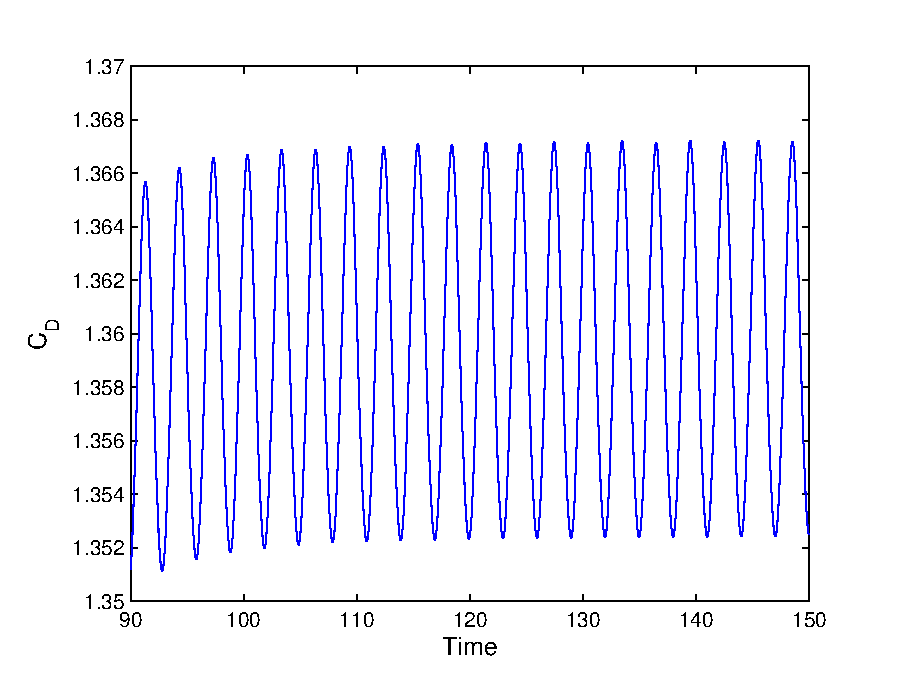
\includegraphics[width=0.45\textwidth]{img/re100dg3cpd60cd90.eps}}
	\end{figure}
\end{frame}
\begin{frame}[allowframebreaks]
	\frametitle{Values for $\text{Re}=200$}
	\begin{columns}
		\column{7cm}
		\scalebox{0.65}{
			\begin{minipage}{\the\textwidth}
			\begin{table}[htp]
				\centering
				\def\arraystretch{1.5}
				%	\begin{minipage}[b]{0.3\textwidth}	
				\begin{tabular}{|c|c|c|c|c|}
					\hline
					\multicolumn{2}{|c|}{\multirow{2}{*}{$C_D$}} & \multicolumn{3}{c|}{CpD} \\ \cline{3-5} 
					\multicolumn{2}{|c|}{}                       & 40     & 60    & 80    \\ \hline
					\multirow{3}{*}{DG}            & 1           &   $0.8144\pm 0.0028$     &     $1.2427 \pm 0.0281$  &     $1.2256 \pm 0.0309$   \\ \cline{2-5} 
					& 2           &     $1.2508 \pm 0.0339$   &   $1.3593 \pm 0.0080$    &     $1.3501 \pm 0.0079$   \\ \cline{2-5} 
					& 3           &      -  &     $1.344 \pm 0.0462$   &     -   \\ \hline
				\end{tabular}
				\caption[$C_D$ Values for Each simulation]{$C_D$ Values for Each Simulation}	
				\label{C_D200}
			\end{table}
			\end{minipage}
		}
		\column{5cm}
		\scalebox{0.65}{
			\begin{minipage}{\the\textwidth}
				\begin{table}[htp]
					\centering
					\def\arraystretch{1.5}
					%	\end{minipage}
					%	\centering
					%	\quad
					%	\begin{minipage}[b]{0.3\textwidth}	
					\begin{tabular}{|c|c|c|c|c|}
						\hline
						\multicolumn{2}{|c|}{\multirow{2}{*}{$C_L$}} & \multicolumn{3}{c|}{CpD} \\ \cline{3-5} 
						\multicolumn{2}{|c|}{}                       & 40     & 60    & 80    \\ \hline
						\multirow{3}{*}{DG}            & 1           &    $\pm 3.2629 \cdot 10^{-5}$    &    $\pm 0.5304$   &    $\pm 0.2789$    \\ \cline{2-5} 
						& 2           &     $\pm 0.5653$   &    $\pm 0.6433$   &     $\pm 0.6376$   \\ \cline{2-5} 
						& 3           &     -   &    $\pm 0.6887$  &    -    \\ \hline
					\end{tabular}
					\caption{$C_L$ Values for Each Simulation}	
					\label{CL200}
					%	\end{minipage} 
				\end{table}
			\end{minipage}
		}
		%	\column{4cm}
		
	\end{columns}
	\begin{center}
		\scalebox{0.7}{
			\begin{minipage}{\the\textwidth}
				\begin{table}[htp]
					\centering
					\def\arraystretch{1.5}
					%	\end{minipage}
					%	\centering
					%	\quad
					%	\begin{minipage}[b]{0.3\textwidth}	
					\begin{tabular}{|c|c|c|c|c|}
						\hline
						\multicolumn{2}{|c|}{\multirow{2}{*}{St}} & \multicolumn{3}{c|}{CpD} \\ \cline{3-5} 
						\multicolumn{2}{|c|}{}                       & 40     & 60    & 80    \\ \hline
						\multirow{3}{*}{DG}            & 1           &    $0$    &    $0.1836$   &    $0.1838$    \\ \cline{2-5} 
						& 2           &     $0.2003$   &    $0.2002$   &     $0.2002$   \\ \cline{2-5} 
						& 3           &     -   &    $0.2002$   &    -    \\ \hline
					\end{tabular}
					\caption{Strouhal Numbers for Each Simulation }	
					\label{Str200}
					%	\end{minipage} 
				\end{table}
			\end{minipage}
		}
	\end{center}
	\begin{figure}
		\vspace{-0.5cm}
		\centering
		\subfloat[Lift Coefficient over Time for $90\,\text{s}<t<150\,\text{s}$]{\includegraphics[width=0.45\textwidth]{img/re200dg3cpd60cl90.eps}}
		\subfloat[Drag Coefficient over Time for $90\,\text{s}<t<150\,\text{s}$]{\includegraphics[width=0.45\textwidth]{img/re200dg3cpd60cd90.eps}}
	\end{figure}
\end{frame}